\documentclass[10pt]{beamer}

\usetheme[progressbar=frametitle]{metropolis}
\usepackage{appendixnumberbeamer}

\usepackage{booktabs}
\usepackage[scale=2]{ccicons}

\usepackage{pgfplots}
\usepgfplotslibrary{dateplot}

\usepackage{xspace}
\newcommand{\themename}{\textbf{\textsc{metropolis}}\xspace}

\title{Dimension Reduction}
\subtitle{Linear Algebra Project Report, Dr.Ramin Javadi}
% \date{\today}
\date{}
\author{MohammadSadegh Akhoundzadeh , Maryam Meghdadi}
\institute{Department of Electrical and Computer Engineering, Isfahan University of Technology}	
% \titlegraphic{\hfill\includegraphics[height=1.5cm]{logo.pdf}}

\begin{document}

\maketitle

\begin{frame}{Table of contents}
  \setbeamertemplate{section in toc}[sections numbered]
  \tableofcontents[hideallsubsections]
\end{frame}

\section{Introduction}

\begin{frame}[fragile]{Introduction}
\textbf{Dimensionality reduction} \textcolor{red}{\textbf{:}} Reducing the number of random variables by obtaining a set of \textcolor{red}{principal variables}
\\
 The higher the number of features \textcolor{red}{\textbf{->}}  the harder it gets to visualize the training set and then work on it 

\begin{itemize}
\item feature selection
\item feature extraction				
\end{itemize}
   
  \begin{figure}
  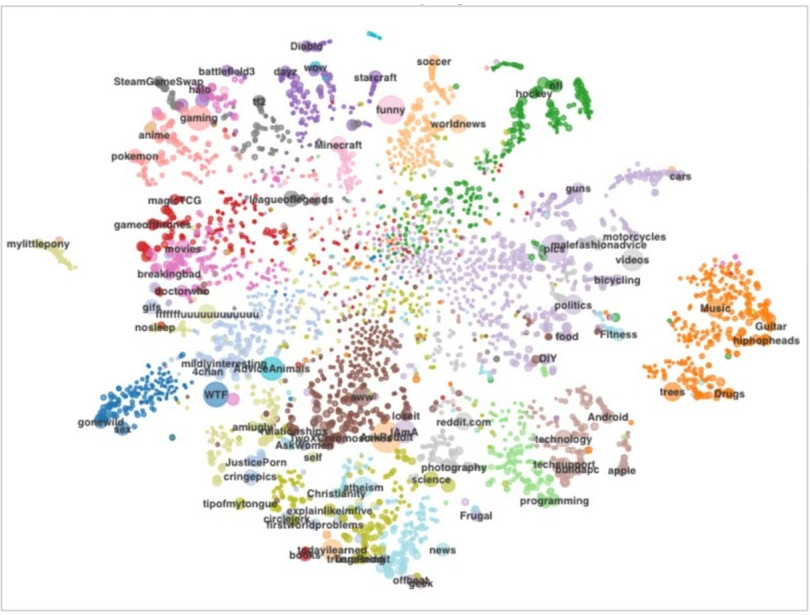
\includegraphics[scale = .22]{1.jpg}
  \end{figure}

\end{frame}

\section{Linear Methods}
\begin{frame}{Linear Methods}
	We discuss and interpret these linear methods: 
	\begin{itemize}
		\item \textbf{PCA}
		\item \textbf{DUAL PCA} 
		\item \textbf{RANDOM PROJECTION} 
		
	\end{itemize}
	
\end{frame}


    \metroset{titleformat frame=smallcaps}
\begin{frame}{Principal Component Analysis (PCA)}
\begin{itemize}
		\item Very popular technique
        \item Find a reduced subspace which  maintains most of the variability of the data ($\hbox{n} \textcolor{red}{\rightarrow} \hbox{d}$) 
        
        \item  d orthogonal vectors that form a new coordinate system which are \textcolor{red}{'principal components'}
	\end{itemize}

\begin{figure}[h]
    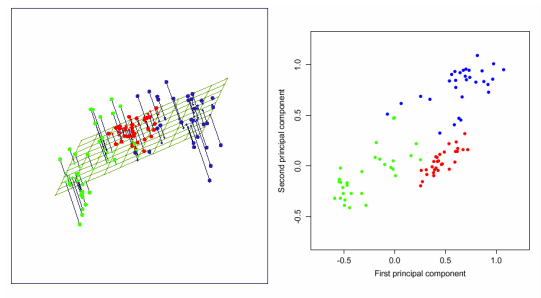
\includegraphics[scale=.4]{pca.png}
    \end{figure}
    
\end{frame} 

    \metroset{titleformat frame=smallcaps}
\begin{frame}{Principal Component Analysis (PCA)}

     $\hbox{Main goal \textcolor{red}{\textbf{:}} find maximum variance } \textcolor{red}{\rightarrow} \hbox{choose first eigenvector $U_1$}$
	Given \textcolor{red}{\textbf{:}} n $\times$ t matrix X and $U_1$ is is a combination of X with $\omega$ coefficients such that $\omega$ = [$\omega_1 \ldots \omega_n$]
    
\begin{equation}
U_1 = \omega^T X 
\end{equation}
\begin{equation}
\text{var}(U_1) = \text{var}(\omega^T X) = \omega^T S \omega
\end{equation}
where S is the n $\times$ n sample covariance matrix of X. 
\begin{center}  
max  $\omega^T$S $\omega$ \space \space s.t. $\omega^T \omega$ = 1 
\end{center}
Using lagrange method and introduce a lagrange multiplier $\lambda$ we have:
\begin{equation}
L(\omega, \lambda) = \omega^T S \omega - \lambda(\omega^T \omega - 1)
\end{equation}
By differentiating L with respect to $\omega$ we have:
\begin{equation}
S\omega = \lambda_1\omega
\end{equation}
\end{frame}

    \metroset{titleformat frame=smallcaps}
\begin{frame}{Principal Component Analysis (PCA)}
Continuing this method for d eigenvectors of covariance matrix S  \textcolor{red}{\textbf{->}} determine the first d principal components
Using SVD  \textcolor{red}{\textbf{->}} obtain these eigenvectors:
\begin{equation}
X = U \Sigma V^T
\end{equation}
where columns of U are eigenvectors of $XX^T$ (covariance matrix).

Algorithm:
We define Y as our projected d-dimensional data (d $<$ n):
\begin{enumerate}
\item {\begin{equation}
Y = U(:, 1:d)^T X \qquad or \qquad Y = U_d^T X
\end{equation}}
\item {Reconstruct the training data:\begin{equation} \hat{X} = U_d Y
\end{equation}}
\item {For a new test example x we compute $y = U^T x$ and then reconstruct it $\hat{x} = U y$ }
\end{enumerate}

\end{frame}	


\metroset{titleformat frame=smallcaps}
\begin{frame}{Dual PCA}
	\begin{itemize}
	\item Very similar to PCA
    \item Faster in the case that the number of features is bigger than the samples
    \item Goal \textcolor{red}{\textbf{:}} reduce dependence of our algorithm on n (the number of features)
    \item Decompose $X^TX$ instead of $XX^T$
    \item  SVD: X = $U\Sigma V^T$ \textcolor{red}{\textbf{->}} $XV = U\Sigma$, where the eigenvectors in U corresponds to nonzero singular values in $\Sigma$.
	\end{itemize}
The top d eigenvectors can be derived:
\begin{equation}
U = XV\Sigma^{-1}
\end{equation}
Replace all uses of U in PCA algorithm.\\
\end{frame}

\metroset{titleformat frame=smallcaps}
\begin{frame}{Dual PCA}
Algorithm:
\begin{enumerate}
\item {Compute Y: \begin{equation} Y = U^TX = \Sigma V^T \end{equation}}
\item {Reconstruct data: \begin{equation}
\hat{X} = UY = U\Sigma V^T = XV\Sigma^{-1}\Sigma V^T = XVV^T \end{equation}}
\item {Project out of sample point x:
\begin{equation}
y = U^T x = \Sigma^{-1} V^T X^T x 
\end{equation}}
\item {Finally reconstruct this sample point:
\begin{equation}
\hat{x} = U y = UU^T x = XV\Sigma^{-2} V^T X^T x 
\end{equation}}
\end{enumerate}
\end{frame}

\metroset{titleformat frame=smallcaps}
\section{Random Projection}

	\begin{itemize}
	\item for the cases with \textcolor{orange}{large number of samples} 
    \item {\textcolor{orange}{What does it guarantee?} \\
    after projecting the points from the \textcolor{red}{n}-dimensional space to \textcolor{red}{K} dimensional space using the randomly drawn matrix W, the \textcolor{red}{distances} between the high dimensional points is \textcolor{red}{preserved} in the lower dimensional projections up to some approximation factor}
	\end{itemize}
This matrix W is:
\[
W[i,j] = \left\{
				\begin{array}{ll}
				+\frac{1}{\sqrt{K}} \qquad \text{with probability 1/2}\\
                -\frac{1}{\sqrt{K}} \qquad \text{with probability 1/2}
				\end{array}
         \right \}
  \]      


\metroset{titleformat frame=smallcaps}
\section{Nonlinear Methods}


\begin{frame}{What's the problem}
	What happen's if we have a manifold ?
    \begin{figure}[h]
    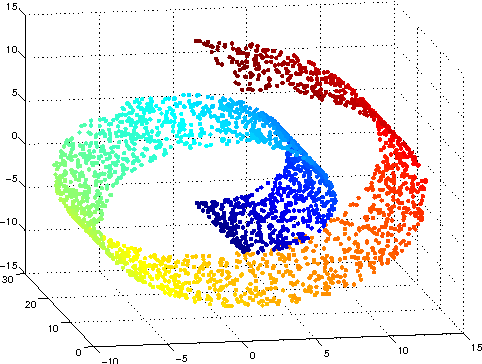
\includegraphics[scale=.4]{manifold.png}
    \end{figure}
    
\end{frame}
\metroset{titleformat frame=smallcaps}
\begin{frame}{Isomap}
	Distance
	\begin{itemize}
		\item Euclidean distance
		\item Geodesic distance
	\end{itemize}
	Algorithm:
	\begin{enumerate}
	\item Construct a k-nearest neighbor graph on n data points
    \item Compute shortest path between all the points (DG) as an estimation of
geodesic distance
	\begin{itemize}
	\item  Dijkstra’s algorithm
    \item  Floyd-Warshall
	\end{itemize}
    \item Compute $k = -\frac{1}{2} H(D^G)^2 H$. find eigenvectors of k and call it V. then find the top p eigenvalues of k and form $\hat{\Lambda}$. The final solution is $Y = {\hat{\Lambda}}^\frac{1}{2} V^T$.
	\end{enumerate}
    
\end{frame}
\metroset{titleformat frame=smallcaps}
\begin{frame}{Laplacian Eigenmap (Spectral Embedding)}
	\begin{enumerate}
	\item 	Using Spectral Clustering 
    \item Affinity Matrix
    \begin{itemize}
    \item \textbf {The neighbourhood graph can be constructed by
finding the k nearest neighbours  and computing the adjacency matrix}
	\item \textbf{Gaussian Distance} 
    \end{itemize}

   \begin{equation}
W_{ij} = e{^{-\frac{||x_i - x_j|| ^ 2}{\gamma}}}
\end{equation} 

	\item Objective Function
    \begin{equation}
\min_{Y} \sum_{i = 1}^{t} \sum_{j = 1}^{t} (y_i - y_j)^2 W_{ij}
\end{equation}
 From spectral clustering we know that:
\begin{equation}
\sum_{i,j} (y_i - y_j)^2 W_{ij} = Y^T L Y 
\end{equation}

    \begin{equation}
	\min_{Y} Tr(YLY^T)  
	\end{equation}
    \begin{center}
 \text{s.t.} $YY^T = I$\\
\end{center}    
	\end{enumerate}
\end{frame}

\section{Experiment}
\begin{frame}{Experiment}
  start by generating three different data to compare the algorithms
  \begin{itemize}
  \item  simple "Hello" in three dimension 
  \item  curved "Hello" 
  \item  S-shape data 
  \end{itemize}
  
 \begin{figure}[htp]

\centering
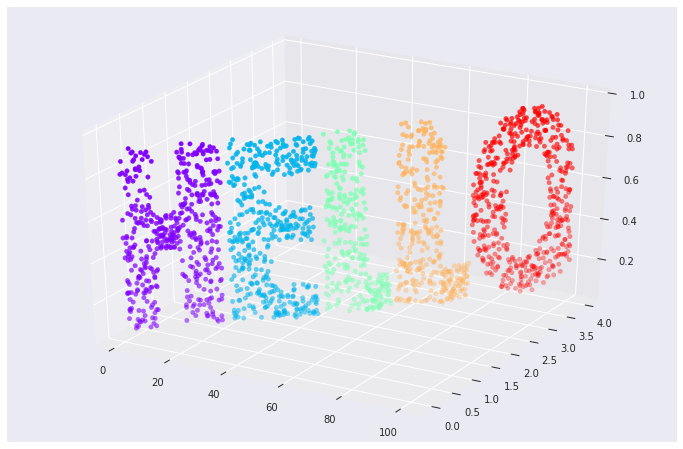
\includegraphics[width=.4\textwidth]{3_dhello_linear_gussian.png}\hfill
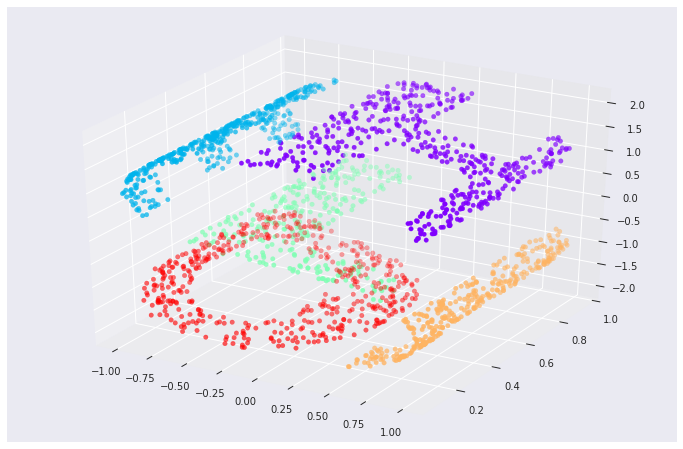
\includegraphics[width=.4\textwidth]{curved_hello.png}
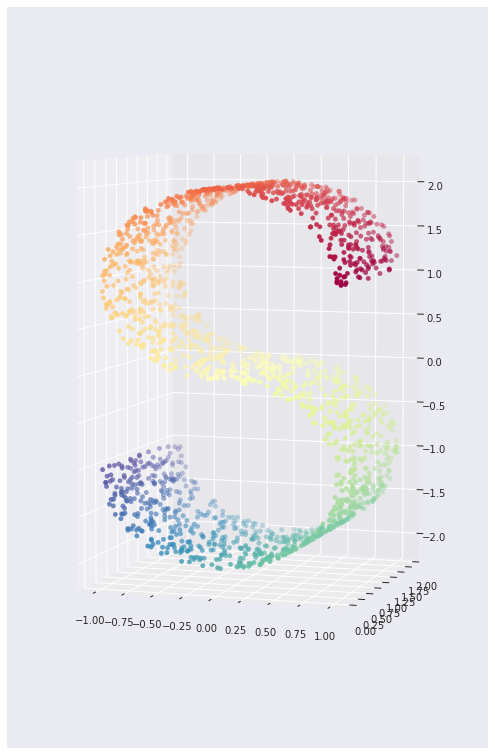
\includegraphics[width=.2\textwidth]{s_3d.png}
\caption{data points that are used}
\end{figure}
\end{frame}

\begin{frame}{The result of algorithms on the first data point}
 \begin{figure}[t]
\centering
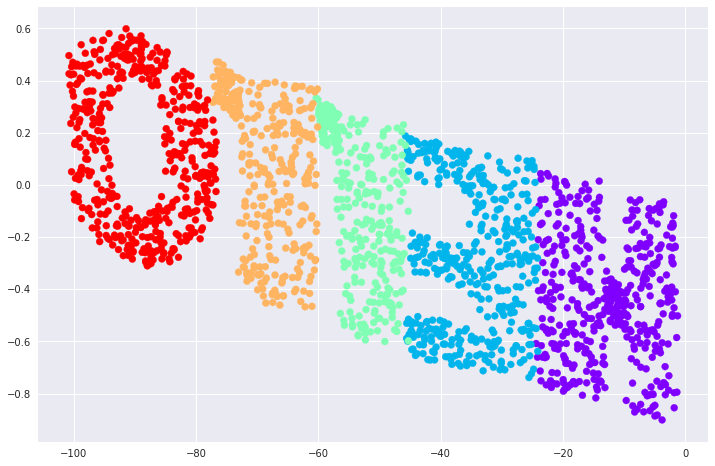
\includegraphics[width=.4\textwidth]{pca_part1.png}\hfill
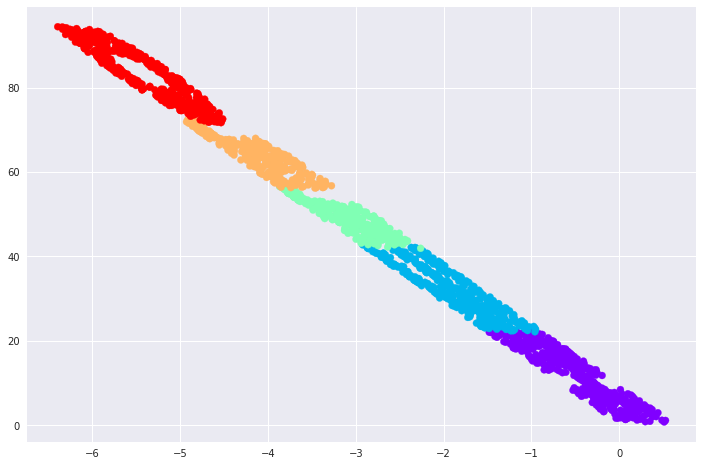
\includegraphics[width=.4\textwidth]{random_projection_part1.png}
\caption{PCA and Random Projection applied to the first data point}
\end{figure}

\begin{figure}[b]
\centering
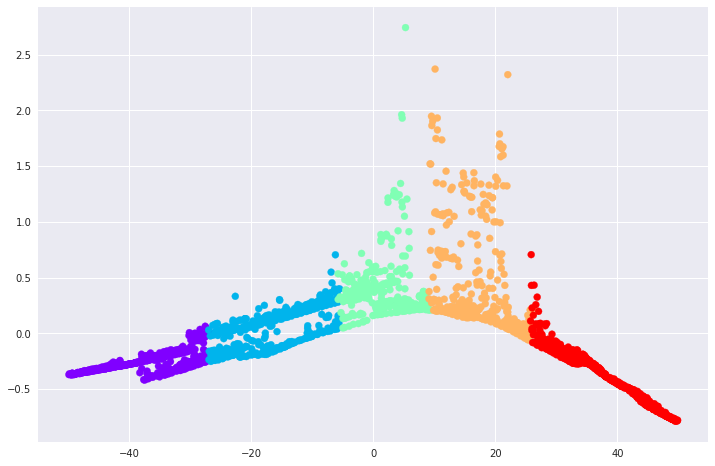
\includegraphics[width=.4\textwidth]{Isomap_part1.png}\hfill
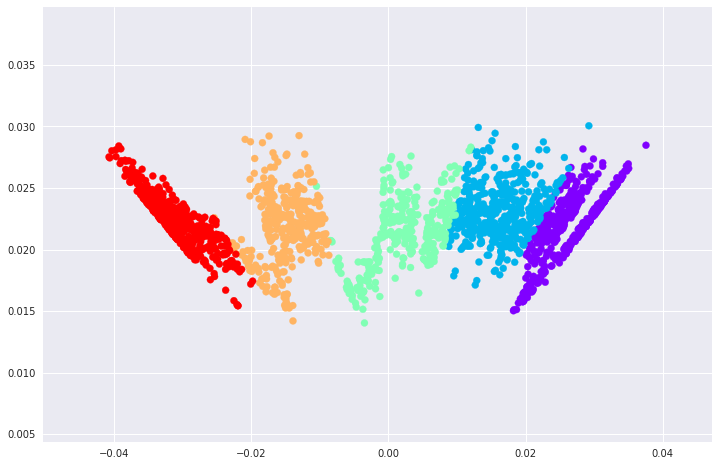
\includegraphics[width=.4\textwidth]{laplacian_part1.png}
\caption{Isomap and Laplacian eigenmap applied to the first data point}
\end{figure}

\end{frame}


\begin{frame}{The result of algorithms on the second data point}
 \begin{figure}[t]
\centering
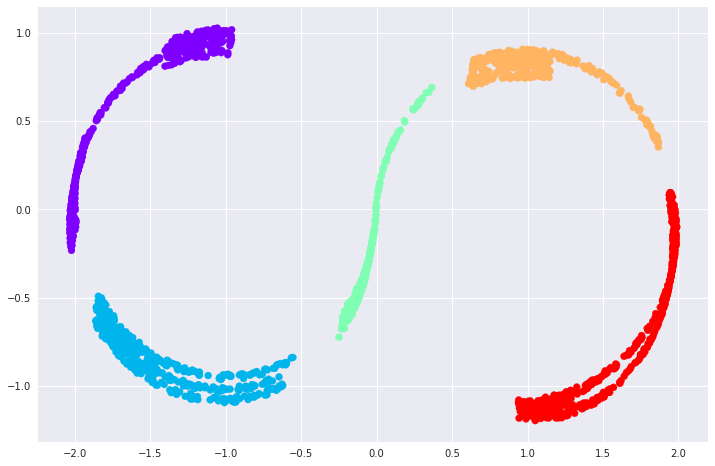
\includegraphics[width=.4\textwidth]{pca_part2.png}\hfill
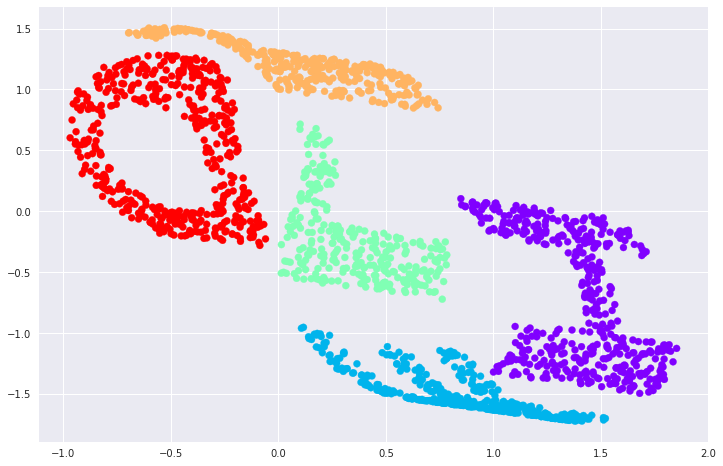
\includegraphics[width=.4\textwidth]{random_projection_part2.png}
\caption{PCA and Random Projection applied to the second data point}
\end{figure}

\begin{figure}[b]
\centering
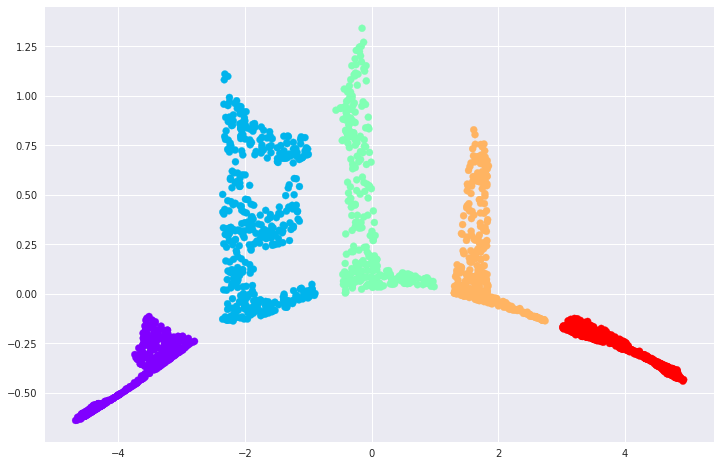
\includegraphics[width=.4\textwidth]{isomap_part2.png}\hfill
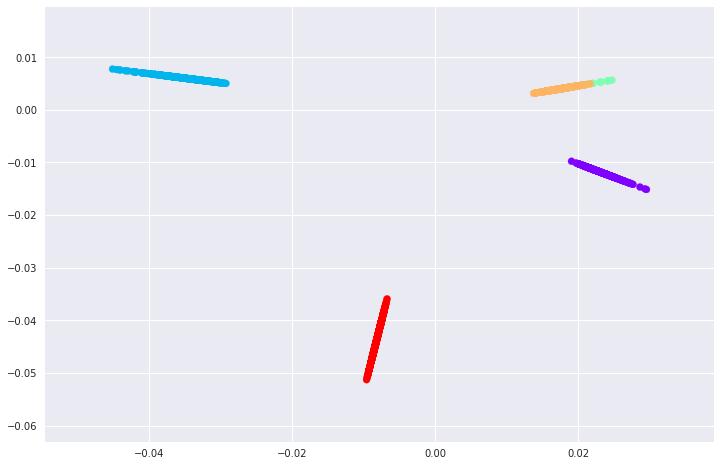
\includegraphics[width=.4\textwidth]{laplacian_part2.png}
\caption{Isomap and Laplacian eigenmap applied to the second data point}
\end{figure}

\end{frame}


\begin{frame}{The result of algorithms on the third data point}
 \begin{figure}[t]
\centering
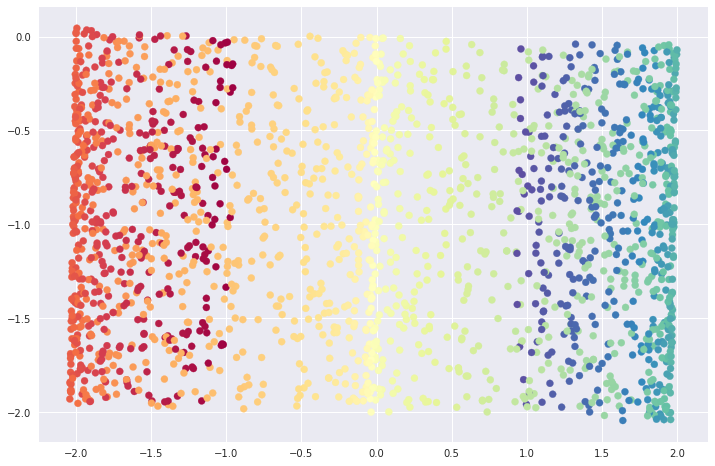
\includegraphics[width=.4\textwidth]{pca_part3.png}\hfill
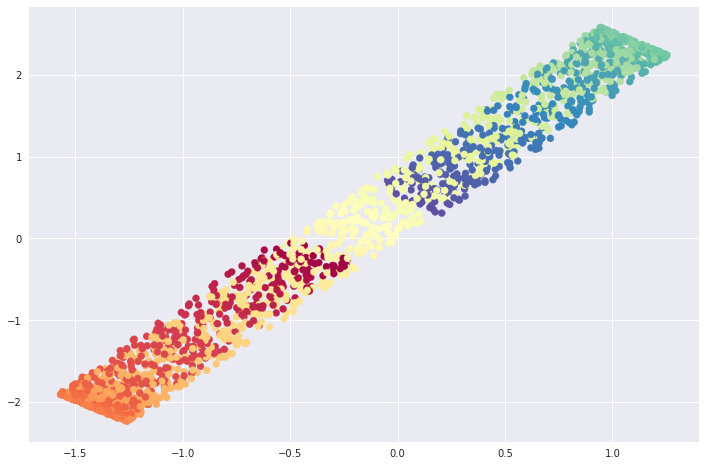
\includegraphics[width=.4\textwidth]{random_projection_part3.png}
\caption{PCA and Random Projection applied to the third data point}
\end{figure}

\begin{figure}[b]
\centering
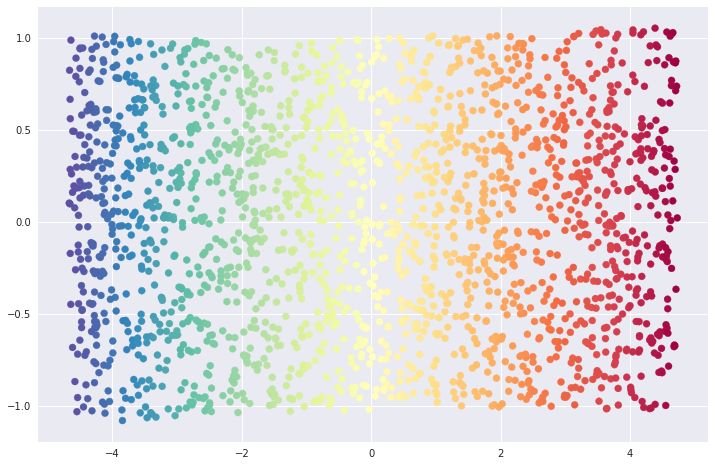
\includegraphics[width=.4\textwidth]{isomap_part3.png}\hfill
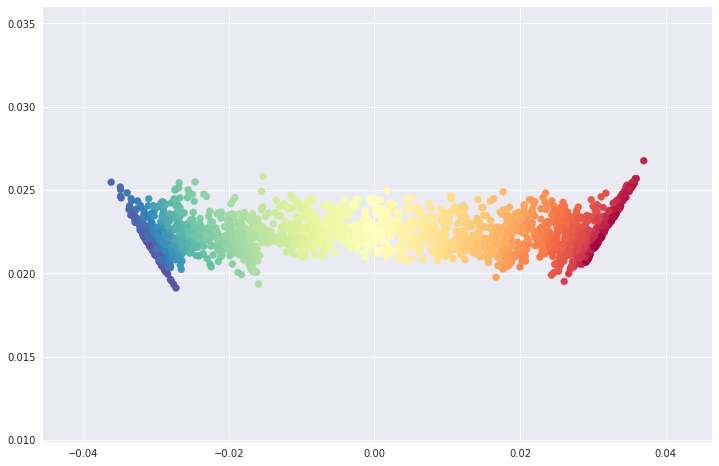
\includegraphics[width=.4\textwidth]{laplacian_part3.png}
\caption{Isomap and Laplacian eigenmap applied to the third data point}
\end{figure}

\end{frame}

\begin{frame}{Source}

  Get the source of the project from here:

  \begin{center}\url{https://github.com/Linear-Algebra-Course/dimension-reduction}\end{center}

  %The theme \emph{itself} is licensed under a
  %\href{http://creativecommons.org/licenses/by-sa/4.0/}{Creative Commons
 % Attribution-ShareAlike 4.0 International License}.

  \begin{center}\ccbysa\end{center}

\end{frame}
\begin{frame}[allowframebreaks]{References}
\cite{Ghodsi2006}
\cite{Kokiopoulou2011}
\cite{Projections}
  \bibliography{Mendeley}
  \bibliographystyle{plain}

\end{frame}

\end{document}
